    \subsection{Resolver \textit{Defects}}\label{sub:defects}

        Nesta secção vão-se explorar a fundo alguns dos \textit{defects} resolvidos durante o período do estágio, incluindo ferramentas e métodos de trabalho e análise utilizados. Este método foi escolhido de forma a que o leitor possa ficar com uma ideia clara do que é necessário e importante no processo do trabalho atribuído, desta forma uma análise profunda pode ser executada evitando uma análise mais supreficial de todas. Para uma visão holística do trabalho, a Tabela \ref{defeitos_trabalhados} detalha todos os \textit{defects} trabalhados, respetivas prioridades.
        
        \begin{table}[htbp] % htbp
            \centering
            \caption{\textit{Defects} Trabalhados}
            \label{defeitos_trabalhados}
            \source{Documentação Interna} % 1- https://impalaintech.com/blog/mendix-vs-outsystems-vs-appian/
            \begin{tblr}{
                % example for tblr: https://tex.stackexchange.com/questions/603349/tabularray-and-new-command-for-multicolumn-cells
                % another example: https://tex.stackexchange.com/questions/605676/tabularray-how-to-control-the-vertical-alignment-of-the-cells-contents
                hlines={lightgray}, vlines={lightgray},
                width = \linewidth,% total width set to width available
                %rows = {c,m}, % c aligns horizontally, m aligns vertically, aligns all rows
                colspec={X[3,c,m] X[3.5,c,m] X[c,m] X[c,m] X[1.2,c,m]},
            }
            % \textbf{Tempo trabalhado}
            \textbf{Título do \textit{defect}} & \textbf{Descrição do \textit{defect}} & \textbf{Prioridade} \\

            % Low, Medium, High, Critical

            ``A Withdrawn FO showing 'Requested' in overview screen \& 'Invalid Data' error message appearing when clicked on 'Requested''' & Um \textit{broker}, ao receber um FO, e esta ser retirada de seguida, o \textit{broker} consegue visualizar ``requested'' na tab ``overview'' para alguns dos UWs. Quando o \textit{broker} clica no estado ``requested'', surge uma mensagem de erro ``Invalid Data''. & Baixa \\

            ``The broker can't find the contract using the filter despite the UMR contract is showing in the filter that exists.'' & Contratos não conseguiam ser encontrados através dos filtros de procura. & Média \\

            ``Regression - Subjectivity email notifications - Wrong emails getting triggered for subjectivity flow'' & Quando o UW apaga uma \textit{subjectivity} com o estado de ``satisfaction pending'', a subjetividade passa para o estado ``Proposed Deletion''. E quando o Broker aceita a proposta de exclusão da \textit{subjectivity}, o e-mail/notificação ``Firm Order - Update'' é acionado em vez do e-mail/notificação ``Subjectivity Deleted''. & Média \\

            ``Amend Master Facility - UW not visible at Overview tab and Sign and Close page'' & O UW não se encontra visível na tab \textit{Overview} quando se efetua uma alteração à MF. & Média \\

            ``PRE - Master Facility - Post Bind Reference or Risk code changes are not showing any stamp details in the transaction logs'' & Ao criar um novo contrato, em certas situações, detalhes dos \textit{stamps} não eram criados. Não foi possível reproduzir. & Média \\

            ``Stamp Visibility | Broker - The UW stamps should be filtered by the company.'' & Refira à Secção \ref{visibilidade_de_stamp_defect} & Média \\

            ``Index out of bounds when submiting cancel and replace'' & Refira à Secção \ref{index_out_of_bounds_defect} & Urgente \\
            \end{tblr}
        \end{table}

        Vamos, primeiramente, detalhar a forma de análise de \textit{defects}:

        \subsubsection{Análise de \textit{Defects}}\label{secsec:analise_de_defects}

            De uma forma geral, os passos na análise e resolução de um \textit{defect} devem seguir os seguintes pontos:

            \begin{enumerate}
                \item A análise começa pela reflexão sobre se o \textit{defect} está contemplado, ou não, nas USs, ou seja, se não será um GAP;
                
                Sendo um GAP, é passado à equipa relevante para a US ser alterada, caso contrário avança-se para o próximo passo: 
                \item De seguida deve-se identificar o ambiente em que se deve testar e resolver o \textit{defect};
                
                Existe um campo ``Target Fix Release'' que indica a release em que o \textit{defect} deverá ser resolvido, esta informação deve ser ligada ao \textit{deployment aggregator} para identificar em qual dos ambientes de desenvolvimento se deve prosseguir, no caso dos ambientes do protótipo da Figura \ref{fig:deployment-aggregator}, os ambientes DED ou DES.  
                \item Deve-se então atualizar o ``Assignee'' para o nosso utilizador na plataforma;
                \item Analisar, preparar e corrigir o \textit{defect} na plataforma Service Studio atualizando sempre o estado no \textit{defect} apropriadamente, neste caso de \textit{New} para \textit{In Analysis} para \textit{Ready For Development} conforme o flow demonstrado na Figura \ref{fig:defect-workflow};
                \item De seguida o mais apropriado será alinhar com os maestros. Para tal será necessário realizar testes e revisões do código e possivelmente retrofit para um ambiente mais a baixo, são também criadas ``subtasks'' para estas tarefas que são, no entanto,  frequentemente realizadas por outras equipas. 
            \end{enumerate}

        \subsubsection{Índice fora dos limites ao submeter \textit{Cancel and Replace}}\label{index_out_of_bounds_defect}

        \textit{Defect} original: ``\textit{Index out of bounds when submiting cancel and replace}''

            % ``defect com a liliana'' no onenote

            Um dos primeiros \textit{defects} analisados, foi analisado em conjunto com um membro da equipa numa dinâmica de \textit{Remote Pair Programming}.

            \textbf{\textit{Pair Programming}}: Também conhecido por \textit{peer programming}, é um estilo de programação ágil onde dois programadores trabalham em conjunto no mesmo dispositivo e no mesmo problema\cite{peer-programming}. Existe debate àcerca do método e da sua eficácia, mas tem sido observado, sendo benéfico, em casos em que a tarefa é complexa e uma alta precisão no código é essencial, bem como em tarefas simples onde o tempo é limitado. É também uma boa forma de aprendizagem e integração, onde participantes reportam resultados positivos em áreas como a aprendizagem, confiança no código, tempo necessário e gosto geral no processo\cite{faja2014evaluating,hannay2009effectiveness}. % \parencites{faja2014evaluating}{hannay2009effectiveness}. 

            \begin{table}[htbp] % 
                \centering
                \caption{Detalhes do defeito '\textit{Index out of bounds when submitting cancel and replace}'}\label{table:defect1}
                \source{Documentação Interna}
                \begin{tabularx}{1\textwidth}{|>{\raggedright\arraybackslash}X|}
                    \hline
                    \rowcolor{lightgray}
                    \textbf{\textit{Defect}} \\
                    \hline
                    \rowcolor{lightgray!20}
                  
                    \begin{quote}
                        \textbf{Descrição do Defeito:}

                        Ao fazer uma correção do tipo \textit{Cancel and Replace}, quando o \textit{broker} submetia a correção ao \textit{underwriter}, aparecia o erro: ``Index out of bounds. Index -1 for bounds [0,0]''.
                        
                        \begin{itemize}
                            \item Resultado Atual: Ocorre o erro: ``Index out of bounds. Index -1 for bounds [0,0]'';

                            \item Resultado Esperado: O \textit{broker} deve ser capaz de enviar a correção ao \textit{underwriter} sem erros;

                            \item Possível Continuar com o Fluxo: Não;

                            \item Solução Alternativa: Não há;

                            \item Passos para Reproduzir:
                            \begin{itemize}
                                \item Criar um \textit{placement} com 1 \textit{underwriter};

                                \item Enviar um pedido de Firm Order;

                                \item Aceitar o pedido de Firm Order;

                                \item O \textit{broker} cria uma correção do tipo \textit{Cancel and Replace};

                                \item Não fazer alterações pelo \textit{Cancel and Replace};

                                \item Submeter o pedido pressionando ``Send Correction to Underwriter'';

                                \item Ao seguir estes passos, o erro ``Índice fora dos limites. Índice -1 para limites [0, 0]'' deve ser exibido.
                            \end{itemize}
                        \end{itemize}
                    \end{quote}

                    \\
                    \hline
                \end{tabularx}
              \end{table}

            \subsubsubsection*{Análise e Resolução:}

                A descrição do \textit{defect} em causa encontra-se na Tabela \ref{table:defect1}. Fazendo a análise segundo a Secção \ref{secsec:analise_de_defects}:

                \begin{enumerate}
                    \item Neste caso, visto que o \textit{defect} se referia a um erro de limites que aparecia na própria plataforma, não foi necessário procurar a US referente à funcionalidade, isto porque facilmente se deduz ser um comportamento causado por um erro no código que não é desejado na lógica de negócio;

                    \item Nesta etapa foram feitos testes que demonstraram que o erro se encontrava apenas num dos ambientes de desenvolvimento, pelo que se procedeu a analisar e resolver o defeito neste ambiente;

                    \item Já se tinha atualizado o ``Assignee'';

                    \item A fase de análise e correção é sempre a mais demorada e imprevisível, sempre atualizando o estado do \textit{defect} quando apropriado:
                    
                    O processo de desenvolvimento e resolução está muito dependente da comunicação com os membros mais adequados da equipa para cada etapa, pelo que grande parte da capacidade de resolução de problemas, especialmente numa fase inicial, depende muito de uma capacidade de comunicação com os colegas de trabalho. 

                    A análise começou com uma troca de informação com uma BA familiarizada com o flow de \textit{cancel and replace} que nos direcionou para a ação com a lista onde provavelmente ocorria o problema.

                    De seguida fomos à ação em causa, ativamos o debugger do Service Studio, fizemos um \textit{cancel and replace} na plataforma e identificamos a causa do problema, como é possível ver na Figura \ref{fig:index_out_of_bounds1}, o ID do contrato chegava vazio à lista. 

                    \begin{figure}[H]
                        \centering
                        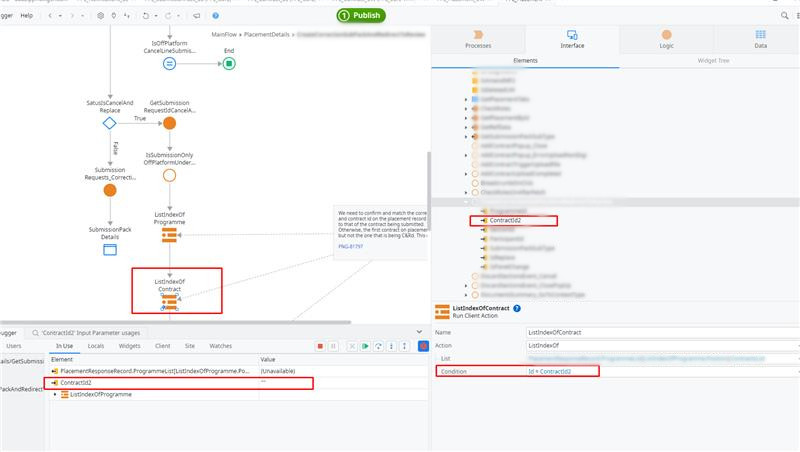
\includegraphics[width=\textwidth]{imgs/IndexOutOfBounds1.jpg}
                        \caption{Index Out of Bounds - Root of the Problem}\label{fig:index_out_of_bounds1}
                        \source{Service Studio Interno}
                    \end{figure}

                    Analisou-se então a interface e de onde vinha o ID do contrato inicialmente ao pressionar o botão, e descobriu-se que o ID era passado ao bloco corretamente. Portanto, era no meio da comunicação, desde quando se clicava no botão até à ação em questão, que se perdia o valor.

                    Os dados eram passados quase exclusivamente de blocos para blocos a partir de \textit{block events}.

                    \textbf{Blocos em OutSystems}: É uma interface reutilizável com código, widgets, ou outros blocos \cite{os-blocks}.

                    \textbf{Eventos de Blocos}: São eventos que permitem ao bloco interagir com o parente do bloco. Estes eventos podem ter variáveis de input ou de output, visto que o ecrã ou o bloco pai não sabe se algo acontece no bloco, como um botão ser clicado, usam-se eventos para passar esta informação para fora, que podem também ser de caráter obrigatório\cite{os-block-events}.

                    Havia uma passagem da informação entre 4 blocos, cujos eventos chamavam diretamente outros eventos, sem haver oportunidade de colocar \textit{breakpoints} no meio do fluxo, depois de uma troca entre um colega acerca do funcionamento de \textit{triggers} em OutSystems, procedeu-se à criação de ações auxiliares que apenas chamavam eventos, e fez-se com que os eventos chamassem estas ações. Desta forma já era possível colocar \textit{breakpoints} e descobrir em que passagem se perdiam os dados. 
                    
                    Veio-se a descobrir que na passagem onde se perdiam os dados, o nome da variável de onde vinham os dados de um bloco era igual ao nome da variável para onde iam os dados noutro bloco, isto normalmente não seria um problema, mas, OS, com o seu código interno em C\#, tem dificuldades em fazer um registo e passagem correta de dados em caso de nomes iguais, pelo que se procedeu à mudança do nome e à publicação da aplicação, o que acabou por solucionar o problema.
                    
                    Retiraram-se então as ações auxiliares e atualizou-se o estado do \textit{defect} adequadamente;
                    
                    \item Nesta etapa comunicou-se com o nosso líder de equipa, e foi necessário reverter as mudanças. O leitor pode-se ter apercebido que o segundo ponto não seguia o padrão de análise de \textit{defects} estabelecido na Secção \ref{secsec:analise_de_defects}. Era necessário analisar o \textit{deployment aggregator} e não apenas resolver o defeito no ambiente de desenvolvimento em que este ocorria. 
                    
                    Veio-se a descobrir que durante aquele período o código de ambas as plataformas de desenvolvimento deveria ser idêntico dado que o código de uma iria substituir a outra brevemente. Pelo que a resolução foi revertida e a análise foi guardada apenas como informação no \textit{defect}, que mais tarde foi usada por um colega que aplicou a resolução na altura e no ambiente correto.
                \end{enumerate}

        \subsubsection{Visibilidade de stamp | Corretora — Os stamps de UW devem ser filtrados pela empresa}\label{visibilidade_de_stamp_defect}

        \textit{Defect} original: ``\textit{Stamp Visibility | Broker - The UW stamps should be filtered by the company}''

            \begin{table}[htbp] % htbp
                \centering
                \caption{Detalhes do defeito '\textit{Stamp Visibility | Broker - The UW stamps should be filtered by the company}'}\label{table:defect2}
                \source{Documentação Interna}
                \begin{tabularx}{1\textwidth}{|>{\raggedright\arraybackslash}X|}
                    \hline
                    \rowcolor{lightgray}
                    \textbf{\textit{Defect}} \\
                    \hline
                    \rowcolor{lightgray!20}
                  
                    \begin{quote}
                        \textbf{Descrição do Defeito:}
                    
                        Um \textit{broker} cria um novo contrato, depois de preencher todas as informações obrigatórias e carregar o documento MRC (documento obrigatório para contratos), seleciona um UW que participará no contrato.
    
                        Se selecionar um UW A (Empresa X), que pertence a várias equipas dentro da Empresa X e Empresa Y (ambas as empresas estão sob a mesma organização), quando seleciona ``Permitted Territory'' - ``Show All'', só devo ver todos os stamps que o UW A tem atribuídos na Empresa X, mas vê-se os stamps atribuídos na Empresa X e Y.
    
                        \begin{itemize}
                            \item Passos para Reproduzir:
                                \begin{itemize}
                                    \item Criar um contrato;
                                    \item Selecionar um UW que pertence a 2 ou mais empresas da mesma organização;
                                    \item Selecionar ``Show All'' no território permitido;
                                    \item Validar se os stamps disponíveis para o \textit{broker} são os stamps atribuídos ao UW dentro dessa empresa.
                                \end{itemize}
                        \end{itemize}
                    \end{quote}

                    \\
                    \hline
                \end{tabularx}
            \end{table}
            
            \subsubsubsection*{Análise e Resolução:}

                A descrição do \textit{defect} encontra-se na Tabela \ref{table:defect2}. Começou-se a análise pela verificação da US associada à funcionalidade, depois de uma troca com um membro da equipa familiarizado com as USs, identificou-se a US da Tabela \ref{table:us1}.

                \begin{table}[H] % htbp
                    \centering
                    \caption{Detalhes da US ``\textit{List of Stamps - Add a Stamp}''}\label{table:us1}
                    \source{Documentação Interna}
                    \begin{tabularx}{1\textwidth}{|>{\raggedright\arraybackslash}X|}
                        \hline
                        \rowcolor{lightgray}
                        \textbf{User Story:} Lista de stamps --- Adicionar um stamp \\
                        \hline
                        \rowcolor{lightgray!20}
                      
                        \begin{quote}
                            \textbf{Visão da User Story:} Para a configuração de um Transportador, os stamps estão vinculados à hierarquia (Organização, Empresa e Utilizador). Esta US permitirá a criação de uma lista de stamps. A lista de stamps também incluirá a ocultação de stamps inativos na lista global.
                        
                            \textbf{Como...} Administrador RIL
                        
                            \textbf{Eu quero...} Adicionar um stamp
                        
                            \textbf{Para quê...} Configurar uma lista de stamps
                        
                            \textbf{Critérios de Aceitação de Negócios:}
                        
                            \textbf{Configuração inicial do ecrã de stamps:}

                            \begin{itemize}
                                \item Dado o Administrador RIL estar no ecrã ``hierarquia'' \newline
                                Quando o Administrador RIL seleciona a aba ``stamps'' \newline
                                Então, a descrição da aba será ``lista de stamps'';

                                \item Dado o Administrador RIL estar na tela ``hierarquia'' \newline
                                Quando o Administrador RIL seleciona a aba ``stamps'' \newline
                                Então, mostra as seguintes colunas de dados (na ordem listada): Nome do stamp, tipo de agência, tipo de stamp, válido a partir de, válido até, estado, classificação e ação;

                                \item Dado o Administrador RIL estar no ecrã ``hierarquia'' \newline
                                Quando o Administrador RIL seleciona a aba ``stamps'' \newline
                                Então, por defeito, mostrar uma lista de carimbos ATIVOS para a organização;
                            
                                \item \textit{etc.}
                            \end{itemize}
                            
                        \end{quote}
                        \\
                        \hline
                    \end{tabularx}
                \end{table}

                Após a análise desta US, deduziu-se que se tratava de um GAP, isto porque na US original dizia ``por defeito, mostrar uma lista de carimbos ATIVOS para a organização'', não implicando que devam ser filtrados por empresa. Esta filtragem não se faz na aplicação, e isso torna-se evidente neste caso em que o utilizador pertence a várias equipas de diferentes empresas da mesma organização.

                Foi então reportado no próprio \textit{defect} e notificadas as equipas relevantes, que continuaram com o problema a partir daí.

            % Outro defect Defect [PNG-74147] Stamp Visibility | Broker - The UW stamps should be filtered by the company. - Jira (atlassian.net)